\problemname{Tycho}

\illustration{.4}{img/MarsPerseveranceRover.jpg}{}

\noindent
Das Planetenerkundungsfahrzeug \emph{Tycho VIII} muss nach dem Sammeln von Mineralproben zur Heimatbasis zurückkehren.
Tycho bewegt sich in einer geraden Linie von Position~$0$ zur Heimatbasis an Position~$b$.
Dabei bewegt er sich mit einer langsamen, aber stetigen Geschwindigkeit von $1$~Einheit pro Sekunde vorwärts.
Jede Sekunde erleidet Tycho $1$~Einheit an Umweltschäden durch die rauen Bedingungen des Planeten.

Die Situation wird durch die Strahlung eines nahe gelegenen Pulsars noch verschlimmert, die alle $p$ Sekunden $d$ zusätzliche Schadenseinheiten verursacht.
Der Strahlungsschaden kann jedoch vermieden werden, indem man in einem von $n$ verschiedenen Verstecken Schutz sucht - Höhlen, Vegetation, große Felsen, Kadaver der Megafauna des Planeten - und sich auf den Weg macht.
Tycho kann sich entscheiden, an einem beliebigen Punkt für eine beliebige Anzahl von Sekunden stillzustehen.

Die Startposition~$0$ und die Heimatbasis bei~$b$ sind beide geschützt, so dass Tycho dort keinen Strahlungsschaden erleidet.

\medskip
Wie hoch ist der minimale Schaden, den Tycho auf seiner Reise zurück zur Heimatbasis erleiden wird?

\section*{Beispiel}

Betrachten wir die Situation, in der sich die Heimatbasis an der Position $18$ befindet und es Schutzräume an den Positionen $8$ und $15$ gibt.

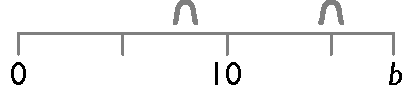
\includegraphics[width=.3\textwidth]{img/samplesetup}

Nehmen wir an, dass die Periode des Pulsars $4$ beträgt, so dass Tycho ohne Schutz zum Zeitpunkt $4$, $8$, $12$ usw. Schaden nehmen würde.
Wenn Tycho von der Startposition (wo er geschützt ist) zum Zeitpunkt $0$ aufbricht, kann er den ersten Schutzraum nach $8$ Sekunden erreichen, wobei er zum Zeitpunkt $4$ Strahlungsschaden $d$ erleidet (aber keinen zum Zeitpunkt $8$, weil er dann geschützt ist).
Setzt er seinen Weg fort, ohne anzuhalten, erreicht er die Heimatbasis zum Zeitpunkt $18$, wobei er $d+d$ weitere Einheiten Strahlungsschaden erleidet (zum Zeitpunkt $12$ bzw. $16$).
Auf diese Weise erleidet er $d+d+d=3d$ Einheiten Strahlungsschaden und $18$ Einheiten Umweltschaden.
Wenn Tycho stattdessen am $2$-ten Bunker (an der Position $15$) eine Sekunde lang wartet, verursacht das Aufblitzen des Pulsars zum Zeitpunkt $16$ keinen Schaden, und er erreicht die Heimatbasis zum Zeitpunkt $19$ mit insgesamt $2d + 19$ Schadenseinheiten.
Dies ist für die meisten Werte von $d$ besser.
Die beiden Situationen sind hier dargestellt:

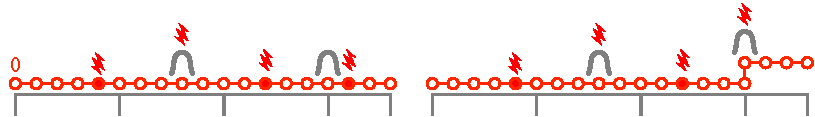
\includegraphics[width=.8\textwidth]{img/sample1_2.pdf}

Wenn der Pulsar eine Periode von $10$ hat, kann Tycho an der Startposition $2$~Sekunden lang warten und dann einfach nach Hause fahren, ohne an einem Schutzraum anzuhalten.
Auf diese Weise passiert er den 1$-ten Schutzraum (an Position~$8$) genau im richtigen Moment, wenn der Pulsar aufblitzt, und erreicht die Heimatbasis zur Zeit $20$, wobei er insgesamt $20$ Umwelt- und keinen Strahlungsschaden erleidet.

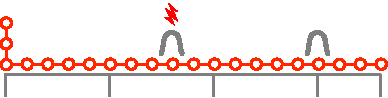
\includegraphics[width=.4\textwidth]{img/sample3.pdf}

\section*{Eingabe}

Die erste Zeile besteht aus vier ganzen Zahlen $b$, $p$, $d$ und $n$, die durch einzelne Leerzeichen getrennt sind:
dem Standort $b$ der Heimatbasis,
die Periode des Pulsars $p$,
der zusätzliche Strahlungsschaden~$d$, der durch jedes Aufblitzen des Pulsars verursacht wird,
die Anzahl~$n$ der Schutzräume.
Die folgenden $n$~Zeilen enthalten jeweils eine ganze Zahl, die die Standorte der Schutzräume $a_1$, $\ldots$, $a_n$ angibt, wobei 
$0<a_1<\cdots <a_n< b$. % constraint:shelterbounds, constraint:sortedshelters

\section*{Ausgabe}

Gib eine einzelne ganze Zahl aus: die Mindestmenge an Schaden, die Tycho erleiden muss, um $b$ zu erreichen.

\section*{Beschränkungen und Bewertung}

Du kannst annehmen, dass
$p < b$ % constraint:pulsehappens
und
$n < b$. % constraint:sheltersfit
Es gilt immer
$1\leq b\leq 10^{12}$, % constraint:b
$0\leq d \leq 10^6$, %constraint:d
und
$0\leq n \leq 10^5$. % constraint:n

Deine Lösung wird in einer Reihe von Testgruppen getestet, von denen jede eine bestimmte Anzahl von Punkten wert ist.
Jede Testgruppe enthält eine Reihe von Testfällen.
Um die Punkte für eine Testgruppe zu erhalten, musst du alle Testfälle in der Testgruppe lösen.
Deine endgültige Punktzahl ist die maximale Punktzahl für eine einzelne Einsendung.

\medskip
\begin{tabular}{lll}
Gruppe & Punkte & Beschränkungen \\\hline
  $1$ & $8$  & $p\leq 10^6$ und Tycho braucht nicht zu warten, \emph{nachdem} er Position~$0$ verlassen hat.$^*$ \\ % constraint:nowait
  $2$ & $5$  & $b\leq 1000$, $p\leq 100$, $n\leq 10$ \\
  $3$ & $7$  & $b\leq 1000$ \\
  $4$ & $15$ & $p\leq 10^6$, $n\leq 1000$\\
  $5$ & $20$ & $p\leq 100$\\
  $6$ & $35$ & $p\leq 10^6$\\
  $7$ & $10$ & \emph{Keine weiteren Beschränkungen}
\end{tabular}

\medskip
\noindent $^*$ In der Testgruppe~$1$ muss Tycho möglicherweise noch an der Position~$0$ warten, \emph{bevor} er sich in Bewegung setzt.
Zum Beispiel gehören die Beispieleingaben $2$, $3$ und $4$ zur Testgruppe~$1$.
